\documentclass{article}

% Language setting
% Replace `english' with e.g. `spanish' to change the document language
\usepackage[english]{babel}
\usepackage{titling}
\usepackage{float}

% Set page size and margins
% Replace `letterpaper' with `a4paper' for UK/EU standard size
\usepackage[letterpaper,top=2cm,bottom=2cm,left=3cm,right=3cm,marginparwidth=1.75cm]{geometry}

% Useful packages
\usepackage{amsmath}
\usepackage{graphicx}
\usepackage[colorlinks=true, allcolors=blue]{hyperref}
\title{OpenEDR Cybersecurity Platform}
\author{Md. Shahrukh Islam \and Md. Sohidul Islam}
\date{\today}

\begin{document}

\maketitle

\section{Introduction}

In an era characterized by the relentless evolution of digital technologies, the security of information systems has never been more critical. As organizations and individuals navigate the digital realm, the OpenEDR cybersecurity platform emerges as a powerful ally, offering a comprehensive and open-source solution for Endpoint Detection and Response (EDR). This report embarks on a journey through the intricate landscape of OpenEDR, unveiling its innovative features and robust capabilities, while also exploring its overarching mission in the realm of cybersecurity.

Cybersecurity concerns have transcended their status as mere considerations; they now stand as imperative elements in the realm of digital defense. OpenEDR is more than just a technological tool; it represents the embodiment of a collaborative community-driven endeavor where knowledge and innovation converge to combat ever-evolving cyber threats.

As the cybersecurity landscape grows increasingly complex, OpenEDR simplifies breach detection, protection, and visibility across a myriad of threat vectors. Its real-time visibility and continuous analysis empower security teams to dissect security events at a granular level, facilitating precise root cause analysis and expediting remediation efforts.

This report will delve into the core components of OpenEDR, unraveling its architecture and exploring its integration with the MITRE ATT\&CK framework. From the basic framework to process hierarchy tracking, OpenEDR provides a holistic view of the threat landscape, enabling organizations to fortify their defenses against a wide array of attack techniques.

Beyond its technical prowess, OpenEDR offers a glimpse into a future where cybersecurity remains accessible, adaptable, and resilient. We explore the capabilities and promise of the OpenEDR cybersecurity platform.

\section{OpenEDR Overview}

OpenEDR is the embodiment of a vision that seeks to address the escalating challenges in the realm of cybersecurity. It stands as an open-source cybersecurity platform with a primary focus on Endpoint Detection and Response (EDR) capabilities. OpenEDR is purpose-built to equip organizations with the tools and capabilities needed for comprehensive security monitoring and incident response.

This platform operates on the principles of transparency and community collaboration. As an open-source project, its source code is openly available to the public, encouraging collective contributions and iterative improvement. OpenEDR represents not just a cybersecurity tool but a testament to the potential of community-driven innovation in the fight against cyber threats.

In the following sections, we will delve into the core components of OpenEDR, shedding light on its architecture and exploring how it aligns with the MITRE ATT\&CK framework. OpenEDR's granular security monitoring, process hierarchy tracking, and real-time visibility capabilities make it a potent instrument in the hands of cybersecurity professionals.

OpenEDR is more than a technological solution; it symbolizes a commitment to evolving cybersecurity practices and fostering a secure digital environment. We navigate through OpenEDR's features and capabilities, unveiling the promise it holds in safeguarding the digital realm.


\section{High Level Overview of the source code}
The source codes for the main functionalities of the EDR system will be discussed below: \\ \\
\textbf{edrav2/iprj/edrdrv :} This directory of the source code contains some very important files for the working of EDR system. Here are some brief overview of the important files in this folder: \\ 
\begin{enumerate}
     \item \textbf{edrdrv.cpp (File):} This is likely the main source code file for the EDR driver, containing the core functionality of the driver.
    \item \textbf{filemon.cpp and filemon.h (Files):} These files are responsible for providing file monitoring functionality within the EDR driver, likely for tracking file system activities.
    \item \textbf{fltport.cpp and fltport.h (Files):} These files are related to filter port communication, often used in Windows drivers for communication between kernel and user-mode components.
    \item \textbf{log.cpp and log.h (Files):} These files contain code for logging and recording events or activities within the EDR driver. This code is designed for logging information and errors within a software component or driver. The logging can be configured with different log levels, and it provides flexibility for logging messages with various levels of detail.
    \item \textbf{netmon.cpp and netmon.h (Files):} These files are related to network monitoring functionality within the EDR driver, basically for tracking network activities. It defines functions and utilities for initializing, finalizing, and interacting with network monitoring resources, including the \texttt{nfwfpdrv.lib} library.
    \item \textbf{objmon.cpp and objmon.h (Files):} These files are related to object monitoring, mainly for tracking and monitoring changes to system objects. It defines functions and callback mechanisms for monitoring and potentially restricting process-related activities.
    \item \textbf{procmon.cpp and procmon.h (Files):} These files are related to process monitoring functionality within the EDR driver, basically for tracking process activities. These files are responsible for applying rules, filtering events, and enforcing security policies.
    \item \textbf{procutils.cpp and procutils.h (Files):} These files contain utility functions related to process management and monitoring.
    \item \textbf{regmon.cpp and regmon.h (Files):} These files are responsible for registry monitoring functionality, mainly for tracking changes to the Windows Registry. Also, they are responsible for features for self-defense, event generation, and rule management. \\
\end{enumerate} 

\textbf{edrav2/iprj/libedr:} This directory of the source code also contains some very important files for the working of EDR system. Here are some brief overview of the important files in this folder: \\
\begin{enumerate}
    \item \textbf{eventenricher.cpp and eventenricher.h (Files):} These files contain code for enriching or enhancing event data as part of an event processing pipeline.
    \item \textbf{eventfilter.cpp and eventfilter.h (Files):} These files contain code related to event filtering, where certain events are selected or filtered based on specific criteria. Events appear to be filtered based on predefined rules (FilterRule) that specify timeouts and hashed fields for event matching. The code calculates hashes of events and their associated data for comparison. Events are associated with processes (ProcId), and a timer mechanism is used to periodically clean up process-related data.
    \item \textbf{outputfilter.cpp and outputfilter.h (Files):} These files contain code for filtering or processing the output data generated by the EDR library.
    \item \textbf{patternsearch.cpp and patternsearch.h (Files):} These files are related to pattern searching or matching within the EDR library, which are for identifying specific patterns or behaviors in data.
    \item \textbf{policy.cpp and policy.h (Files):} These files contain code for managing policies within the EDR library, which are sets of rules or configurations governing its behavior.
\end{enumerate}


\section{Key Features}
\begin{enumerate}

    
    \item \textbf{Open Source and Community-Driven:}  OpenEDR is an open-source project with its source code openly available to the public. This approach encourages community involvement and collaboration to improve the platform's capabilities and security.
    
    \item \textbf{Granular Security Monitoring:} This platform offers granular security monitoring capabilities, allowing organizations to analyze security events at the base-security-event level. This granularity is essential for accurate root cause analysis and faster, more effective remediation of security incidents.
    \item \textbf{Continuous Monitoring of Endpoints:} EDR solutions continuously monitor endpoints, such as computers, servers, and mobile devices, for any suspicious or malicious activities. This ongoing surveillance helps identify security issues in real-time.
    
    \item \textbf{Vulnerability Detection:} EDR systems are designed to detect vulnerabilities in endpoint systems. They can identify security weaknesses, outdated software, misconfigurations, or unpatched systems that could be exploited by attackers.
    
    \item \textbf{Alert Generation for Suspicious Activity:} EDR solutions generate alerts and notifications when they detect any behavior or activity on an endpoint that deviates from the normal or expected patterns. These alerts are crucial for early threat detection.
    
    \item \textbf{Customized Alert Generation Mechanism:} EDR platforms often allow organizations to customize alerting and notification mechanisms to match their specific security policies and incident response procedures. This flexibility enables organizations to tailor alerts to their unique needs.
    
    \item \textbf{Event Logging and Log Information:} EDR systems maintain detailed event logs and information related to endpoint activities. These logs provide a historical record of what has happened on an endpoint, which is valuable for forensic analysis and incident response.
    
    \item \textbf{Antivirus Capabilities:} Some EDR solutions incorporate antivirus or anti-malware features. They can detect and mitigate known malware threats, providing an additional layer of defense against common attacks.

    
    \item \textbf{Process Hierarchy Tracking:} OpenEDR provides process hierarchy tracking, which helps in conveying actionable knowledge about security events. It collects detailed information about endpoints, hashes, and both base and advanced events, enabling organizations to understand and respond to security threats effectively.
    
    \item \textbf{Security Architecture:} OpenEDR's security architecture simplifies breach detection, protection, and visibility across various threat vectors. It does this without requiring additional agents or solutions. The platform records telemetry information locally on endpoints and can send this data to locally hosted or cloud-hosted ElasticSearch deployments.
    
    \item \textbf{Real-Time Visibility and Analysis:}  Real-time visibility and continuous analysis are emphasized in OpenEDR. This capability allows organizations to monitor and analyze security events across their environment at a granular level, leading to accurate root cause analysis and improved remediation.
    
    \item \textbf{MITRE Framework Integration:}  OpenEDR integrates with the MITRE ATT\&CK framework, providing organizations with comprehensive attack vector visibility. This alignment with MITRE's framework helps organizations understand and defend against various attack techniques effectively.
\end{enumerate}
\section{Components of OpenEDR}
The OpenEDR cybersecurity platform is comprised of various components that work together to provide comprehensive security monitoring and incident response capabilities. These components can be categorized into runtime components and the installer.

\subsection{Runtime Components}
OpenEDR's runtime components form the core of the platform, providing essential functionality for security monitoring and response. These components include:

\begin{itemize}
    \item \textbf{Core Library:} The basic framework of OpenEDR.
    \item \textbf{Service:} A service application that manages various aspects of the platform.
    \item \textbf{Process Monitor:} Components responsible for per-process monitoring.
        \begin{itemize}
            \item \textbf{Injected DLL:} A library injected into different processes to hook API calls for monitoring.
            \item \textbf{Loader for Injected DLL:} A driver component that loads the injected DLL into each new process.
            \item \textbf{Controller for Injected DLL:} A service component that facilitates interaction with the Injected DLL.
        \end{itemize}
    \item \textbf{System Monitor:} A generic container for various kernel-mode components.
    \item \textbf{File-system Mini-filter:} A kernel component that hooks I/O requests to the file system.
    \item \textbf{Low-level Process Monitoring Component:} Monitors processes creation/deletion using system callbacks.
    \item \textbf{Low-level Registry Monitoring Component:} Monitors registry access using system callbacks.
    \item \textbf{Self-protection Provider:} Prevents unauthorized changes to EDR components and configuration.
    \item \textbf{Network Monitor:} A network filter for monitoring network activity.
\end{itemize}

These runtime components work together to provide a robust and granular security monitoring and response solution.

\subsection{Installer}
The installer component facilitates the deployment of OpenEDR on systems. It ensures that the platform is correctly set up and configured for effective security monitoring and incident response. Generic high-level interaction diagram for runtime components
\begin{figure}[H]
    \centering
    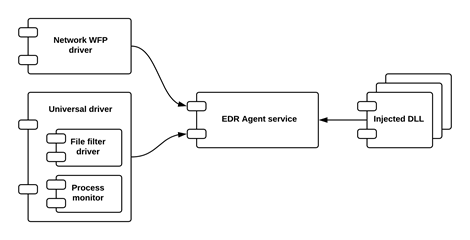
\includegraphics[width=1\textwidth]{interaction-diagram.png}
    \caption{Generic high-level interaction diagram for runtime components}
    \label{fig:interaction_diagram}
\end{figure}



\section{Documentation to Run Each Feature}

In this section, we provide documentation on how to run each feature of the OpenEDR cybersecurity platform. Follow the instructions below to utilize these features effectively.

\subsection{Detection of Suspicious PowerShell Execution}

One crucial aspect of Endpoint Detection and Response (EDR) solutions is their ability to detect suspicious activities, including the execution of PowerShell scripts, which can be a common vector for cyberattacks. To illustrate the detection process, consider the following scenario involving the launch of a script from the ProgramData directory:

\subsubsection{Example of Suspicious Script Launch}

To detect suspicious PowerShell script execution, follow these steps:

\begin{enumerate}
    \item \textbf{Create a Simple Test Script File:} Create a simple test PowerShell script file, e.g., \texttt{test\_script.ps1}, in a known directory.
    
    \item \textbf{Move the Script to ProgramData:} Move the test script (\texttt{test\_script.ps1}) to the ProgramData directory. This directory is often used by legitimate software but can also be exploited by malicious actors.
    
    \item \textbf{Execute PowerShell Script:} Open a Command Prompt with administrative privileges. Execute the following command to run the script from the ProgramData directory:
    
    \begin{verbatim}
    powershell.exe -ExecutionPolicy Bypass -File 
    C:\\ProgramData\\test_script.ps1
    \end{verbatim}
    
    The \texttt{-ExecutionPolicy Bypass} flag is used to bypass PowerShell's execution policy, which might otherwise prevent the execution of scripts. This flag is often seen in attacks where malicious scripts are run.
    
    \item \textbf{Monitor EDR Alerts:} Monitor EDR platform for any alerts or notifications related to script execution from the ProgramData directory. EDR solutions can raise alerts when they detect suspicious activities, providing security teams with insights into potential threats.
\end{enumerate}

This scenario demonstrates how EDR solutions can detect and generate alerts for potentially malicious activities, such as executing PowerShell scripts from directories commonly associated with malware or unauthorized scripts.

\subsection{Detection of Clearing Security Log}

Endpoint Detection and Response (EDR) solutions play a pivotal role in monitoring and identifying potentially malicious activities on endpoints. One such critical activity is the clearing of security event logs, which can be a sign of unauthorized or malicious actions. To demonstrate the detection process, consider the following scenario involving the clearing of the Security event log:

\subsubsection{Scenario}

To detect the clearing of the Security event log and verify EDR detection, follow these steps:

\begin{enumerate}
    \item \textbf{Open PowerShell with Administrative Privileges:} 
    - Open a PowerShell window with administrative privileges. Administrative access is required to perform actions that affect system logs.
    
    \item \textbf{Clear the Security Event Log:} 
    - Use the `wevtutil.exe' utility to clear the Security event log. Execute the following command in the PowerShell window:

      \begin{verbatim}
    echo powershell wevtutil cl Security
    \end{verbatim}
 
    This command clears the Security event log, which contains records of security-related events.
    
    \item \textbf{Verify EDR Detection:} 
    - Monitor the EDR platform for any alerts or notifications related to the clearing of the Security event log. EDR solutions can generate alerts when they detect actions that tamper with system logs.
    
    - Review the EDR platform's logs or alerts to confirm that it has detected the clearing of the Security event log. This detection is critical for identifying potential security incidents.
\end{enumerate}

This scenario illustrates how EDR solutions can be instrumental in detecting and alerting on actions that impact system logs, such as the clearing of the Security event log. By monitoring for such activities, organizations can enhance their security posture and respond promptly to potential threats.


\subsection{Detection of Writing a Fake System File}

Endpoint Detection and Response (EDR) solutions are instrumental in identifying and alerting on suspicious activities, including attempts to create fake system files. To illustrate the detection process, consider the following scenario involving the creation of a fake system file:

\subsubsection{Scenario}

To detect the writing of a fake system file and verify EDR detection, follow these steps:

\begin{enumerate}
    \item \textbf{Open a Command Prompt or PowerShell Window with Administrative Privileges:} 
    - Open a Command Prompt or PowerShell window with administrative privileges. Administrative access is required to perform actions that impact system files.
    
    \item \textbf{Attempt to Create a Fake System File:} 
    - In the administrative Command Prompt or PowerShell window, attempt to create a fake system file in a directory that the EDR platform is monitoring. For example, execute the following command:

    \begin{verbatim}
    echo "Fake svch0st.exe" > C:\Windows\System32\svch0st.exe
    \end{verbatim}

    This command creates a text file named ``svch0st.exe" in the ``C:\textbackslash
\textbackslash Windows\textbackslash\textbackslash System32" directory. The filename is designed to mimic a legitimate system file (``svchost.exe").
    
    \item \textbf{Monitor EDR Alerts:} 
    - Monitor the EDR platform for alerts or notifications related to suspicious file creations that match the file path ``C:\textbackslash
\textbackslash Windows\textbackslash
\textbackslash System32\textbackslash
\textbackslash svchost.exe." EDR solutions can generate alerts when they detect actions that attempt to manipulate or create files in system directories.
    
    - Review the EDR platform's logs or alerts to confirm whether it has detected the creation of the fake system file. Such detections are crucial for identifying potential security threats, especially attempts to tamper with system files.
\end{enumerate}

This scenario demonstrates how EDR solutions can play a critical role in detecting and alerting on actions that involve the creation of fake system files, which could be indicative of malicious intent. By actively monitoring for such activities, organizations can bolster their security defenses and respond swiftly to potential threats.

This is the scenario that escribe the scenario of attempting to create a fake system file and monitoring EDR for alerts related to suspicious file creations.




\begin{figure}[H]
    \centering
    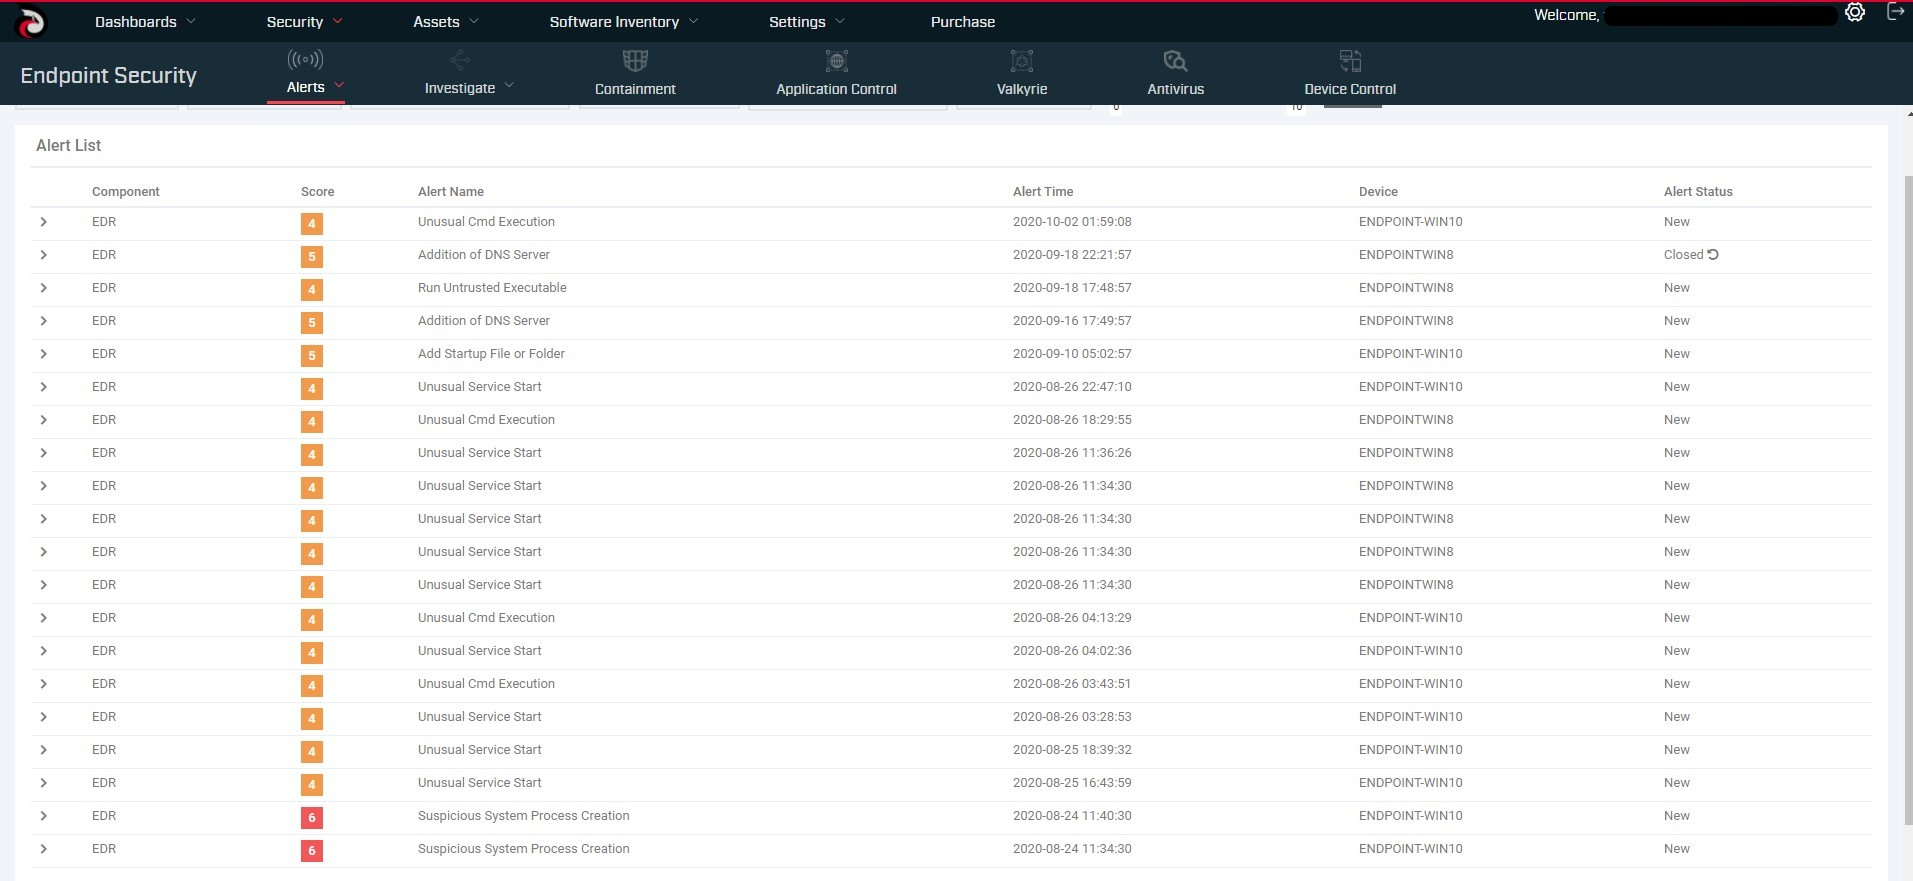
\includegraphics[width=1\textwidth]{Alerting.jpg}
    \caption{Detection / Alerting}
    \label{fig:alerting}
\end{figure}

\begin{figure}[H]
    \centering
    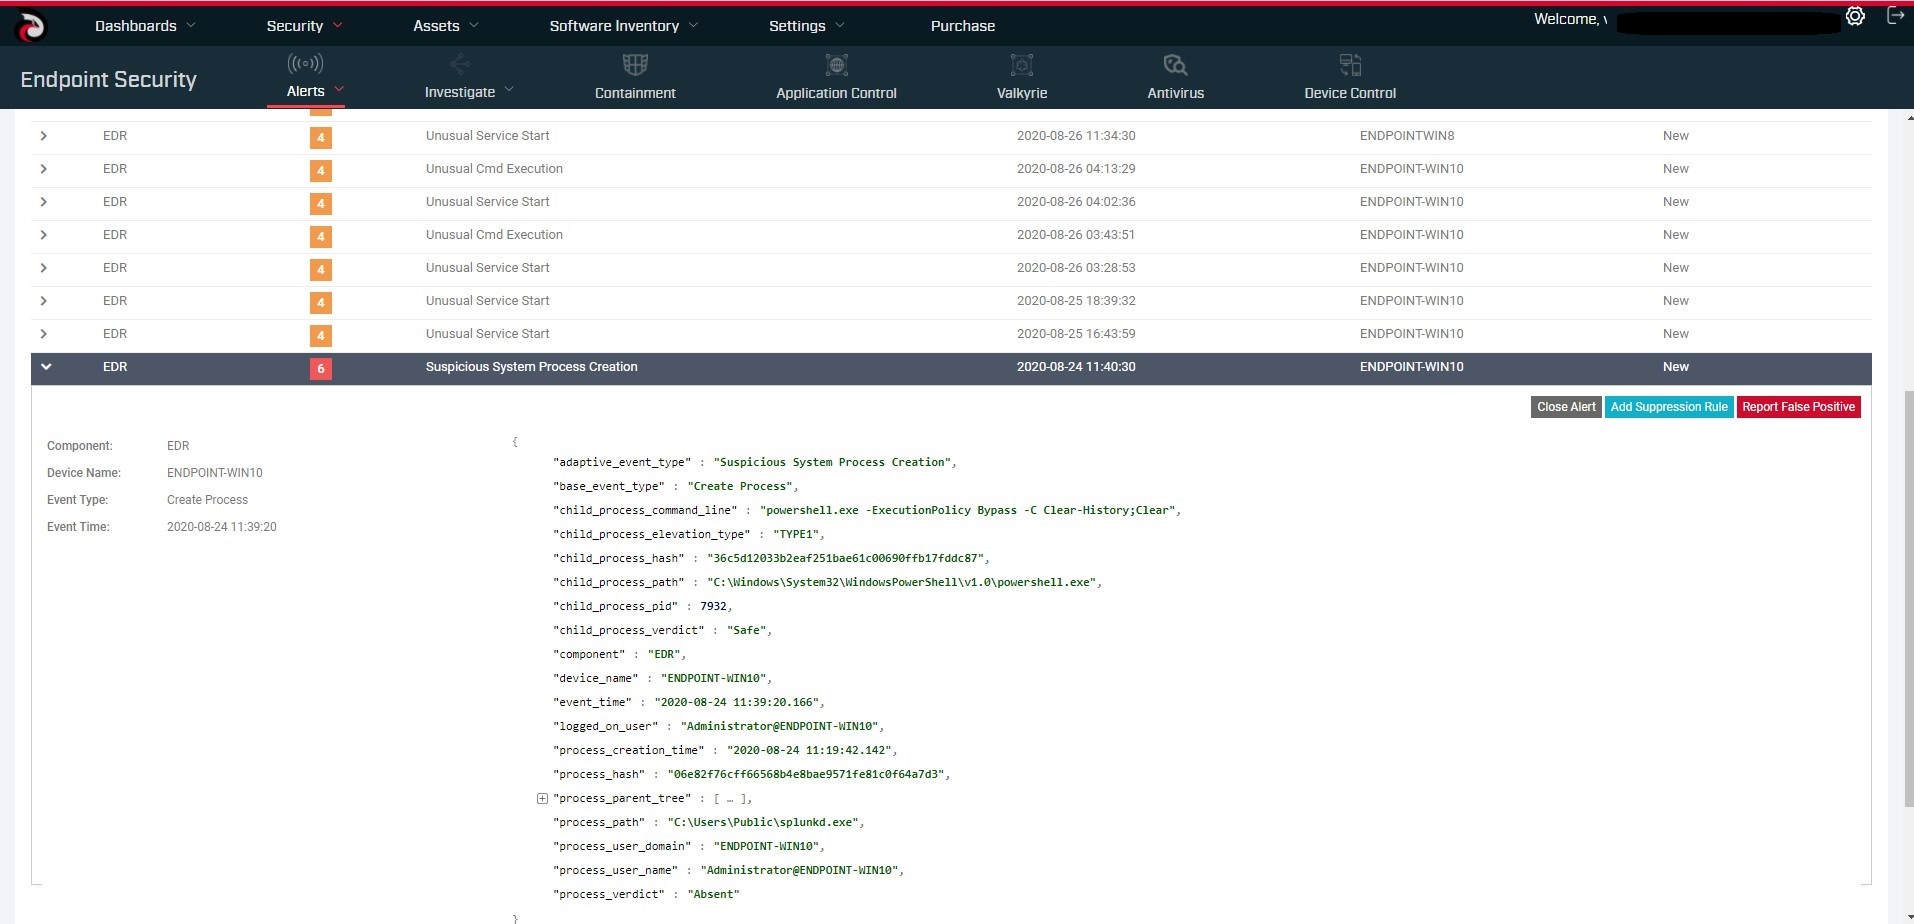
\includegraphics[width=1\textwidth]{Event-details.jpg}
    \caption{Event Details}
    \label{fig:event-detials}
\end{figure}

\begin{figure}[H]
    \centering
    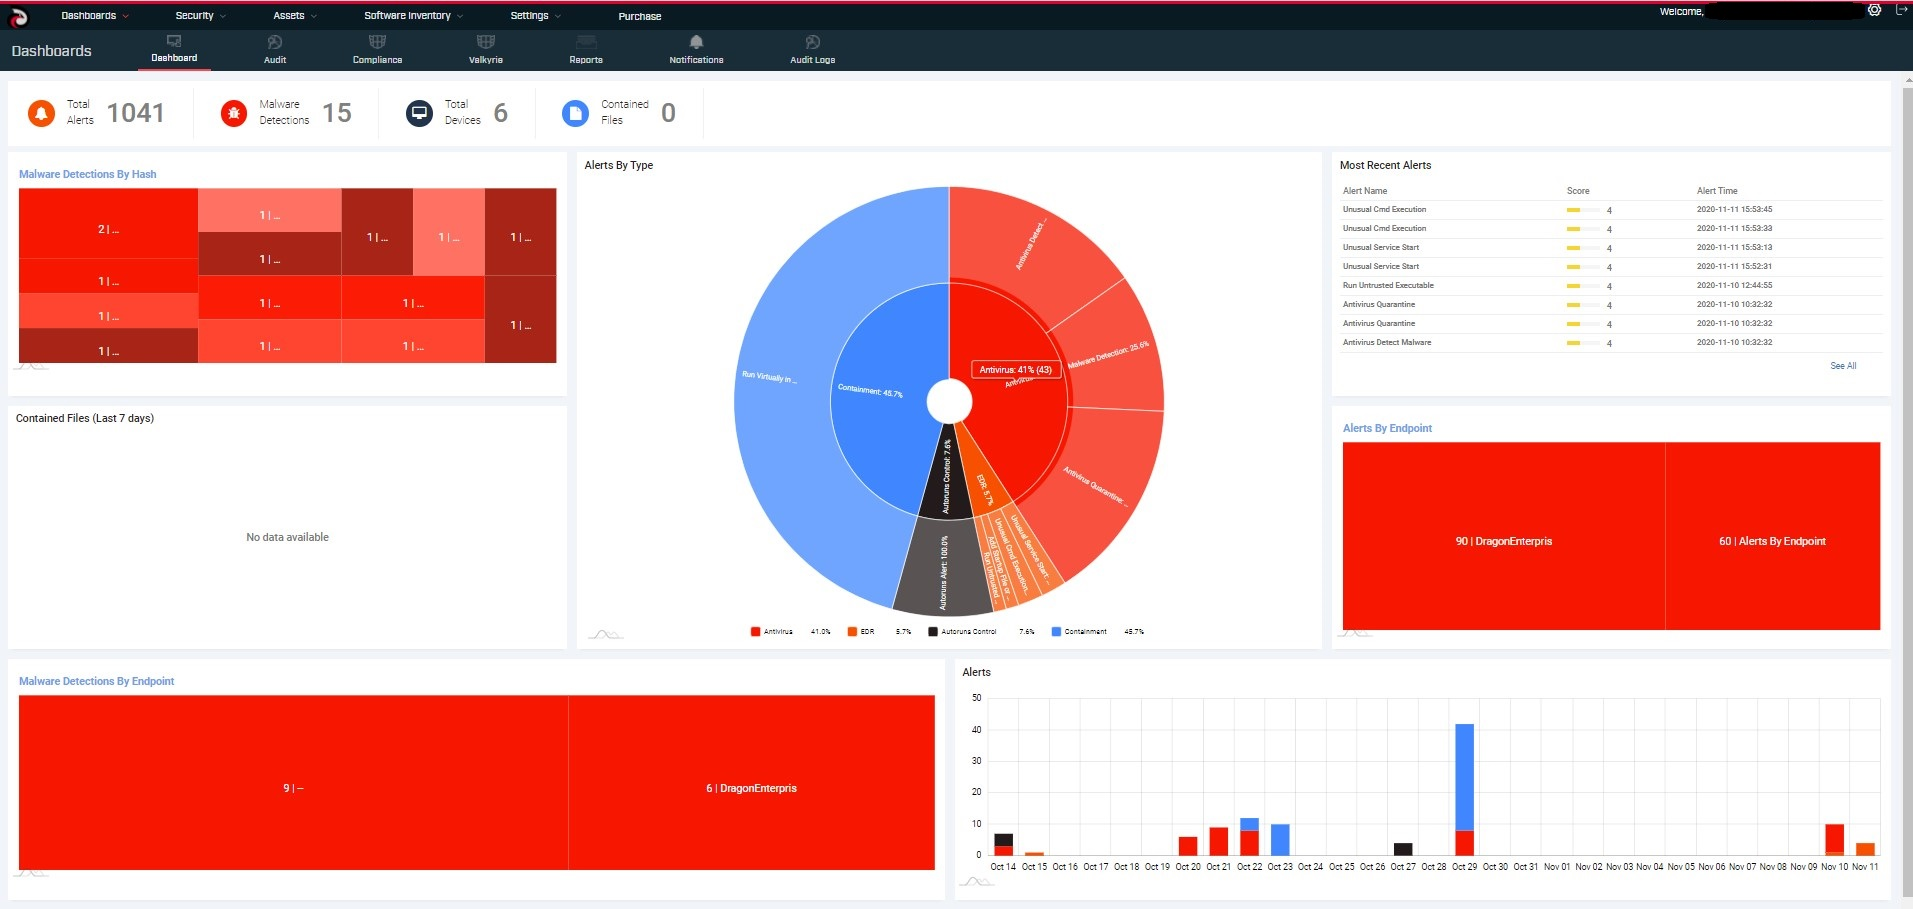
\includegraphics[width=1\textwidth]{Dashboard.jpg}
    \caption{Dashboard}
    \label{fig:dashboard}
\end{figure}

\begin{figure}[H]
    \centering
    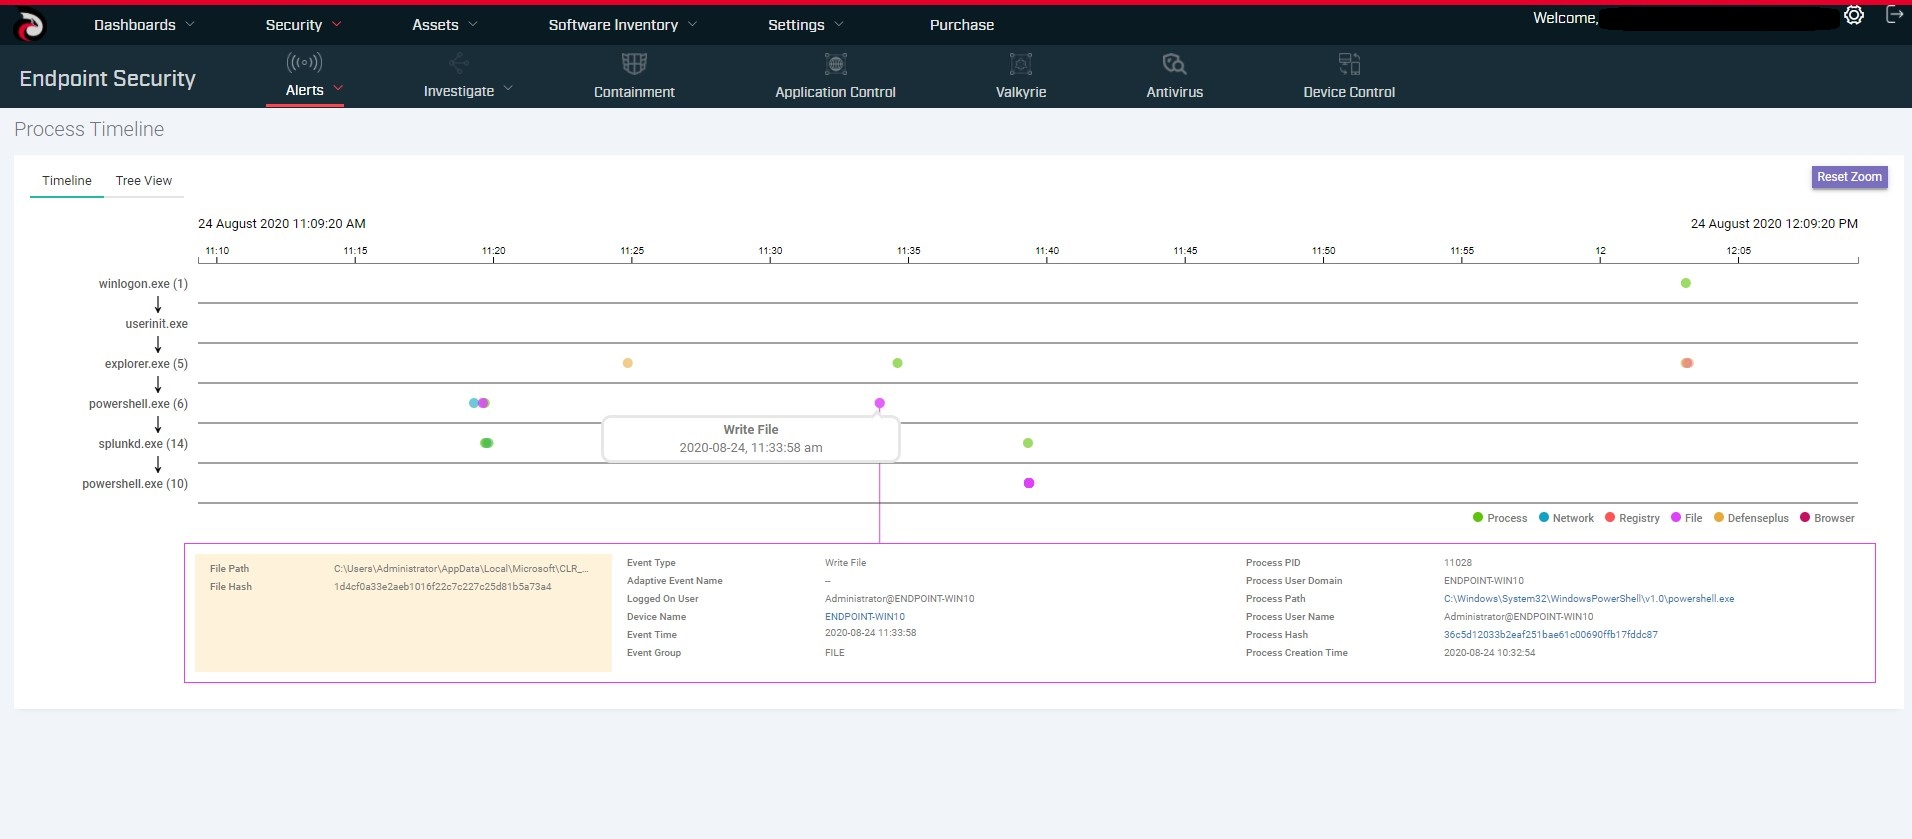
\includegraphics[width=1\textwidth]{Process-timeline.jpg}
    \caption{Process-timeline}
    \label{fig:process-timeline}
\end{figure}



\begin{figure}[H]
    \centering
    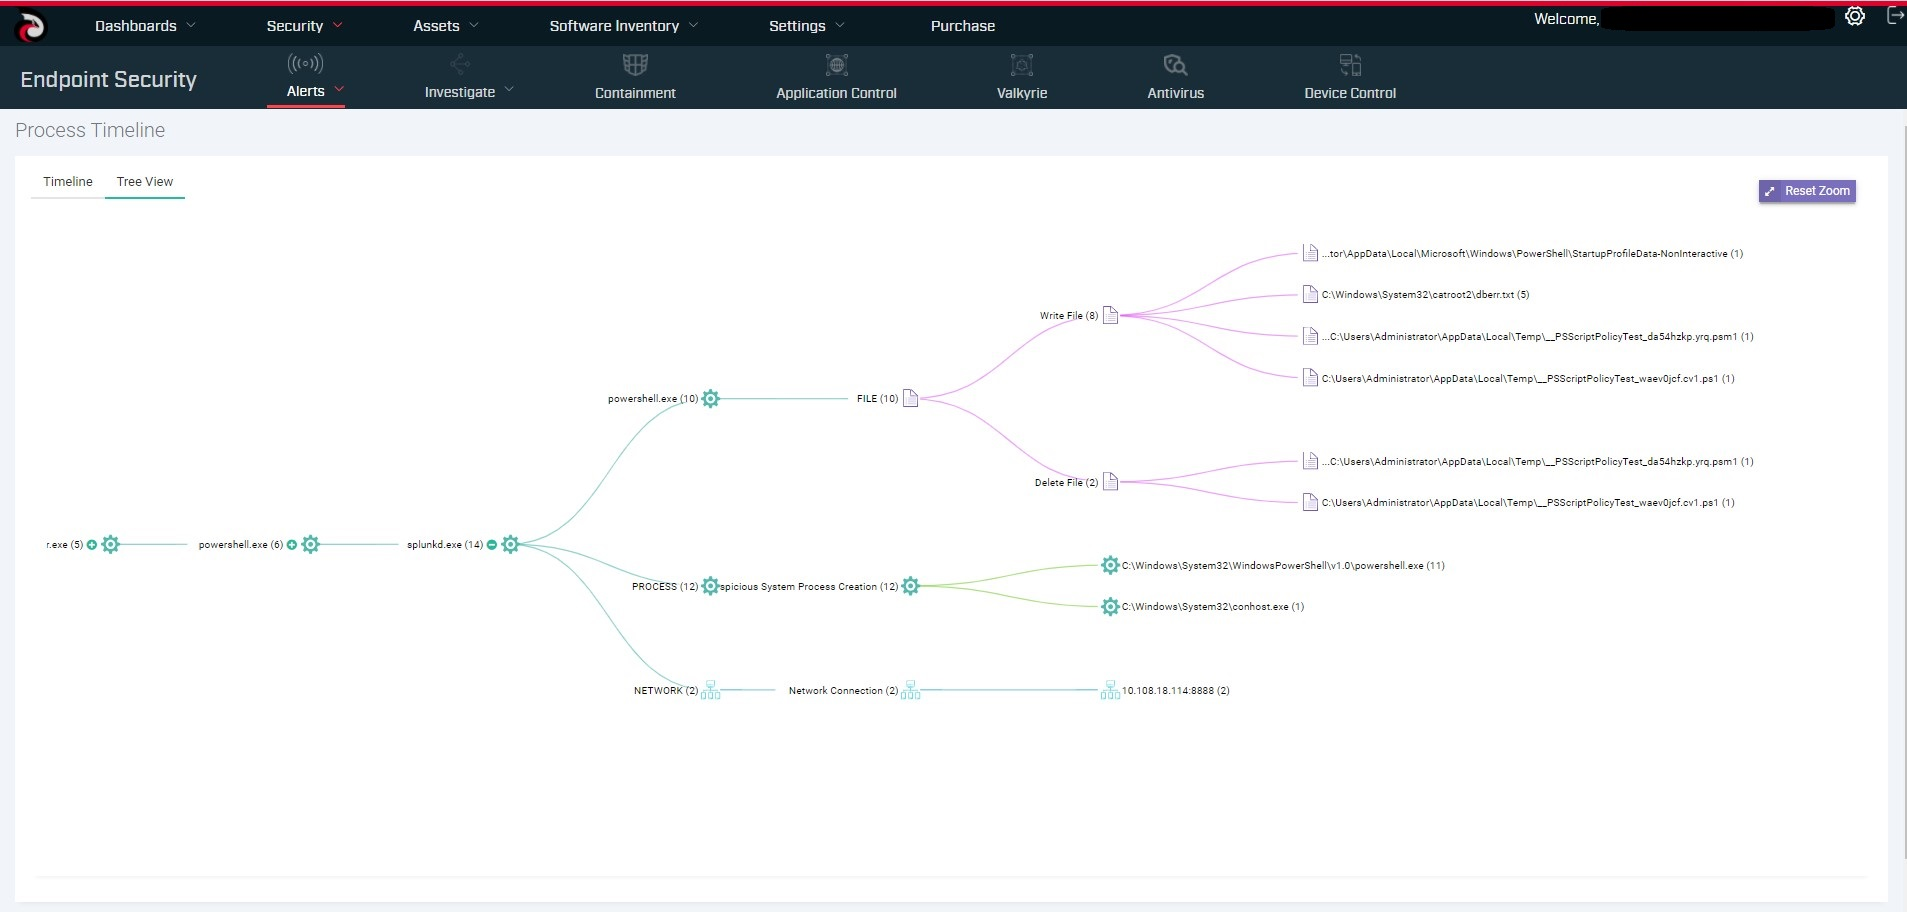
\includegraphics[width=1\textwidth]{Process-treeview.jpg}
    \caption{Process-treeview}
    \label{fig:process-treeview}
\end{figure}


\begin{figure}[H]
    \centering
    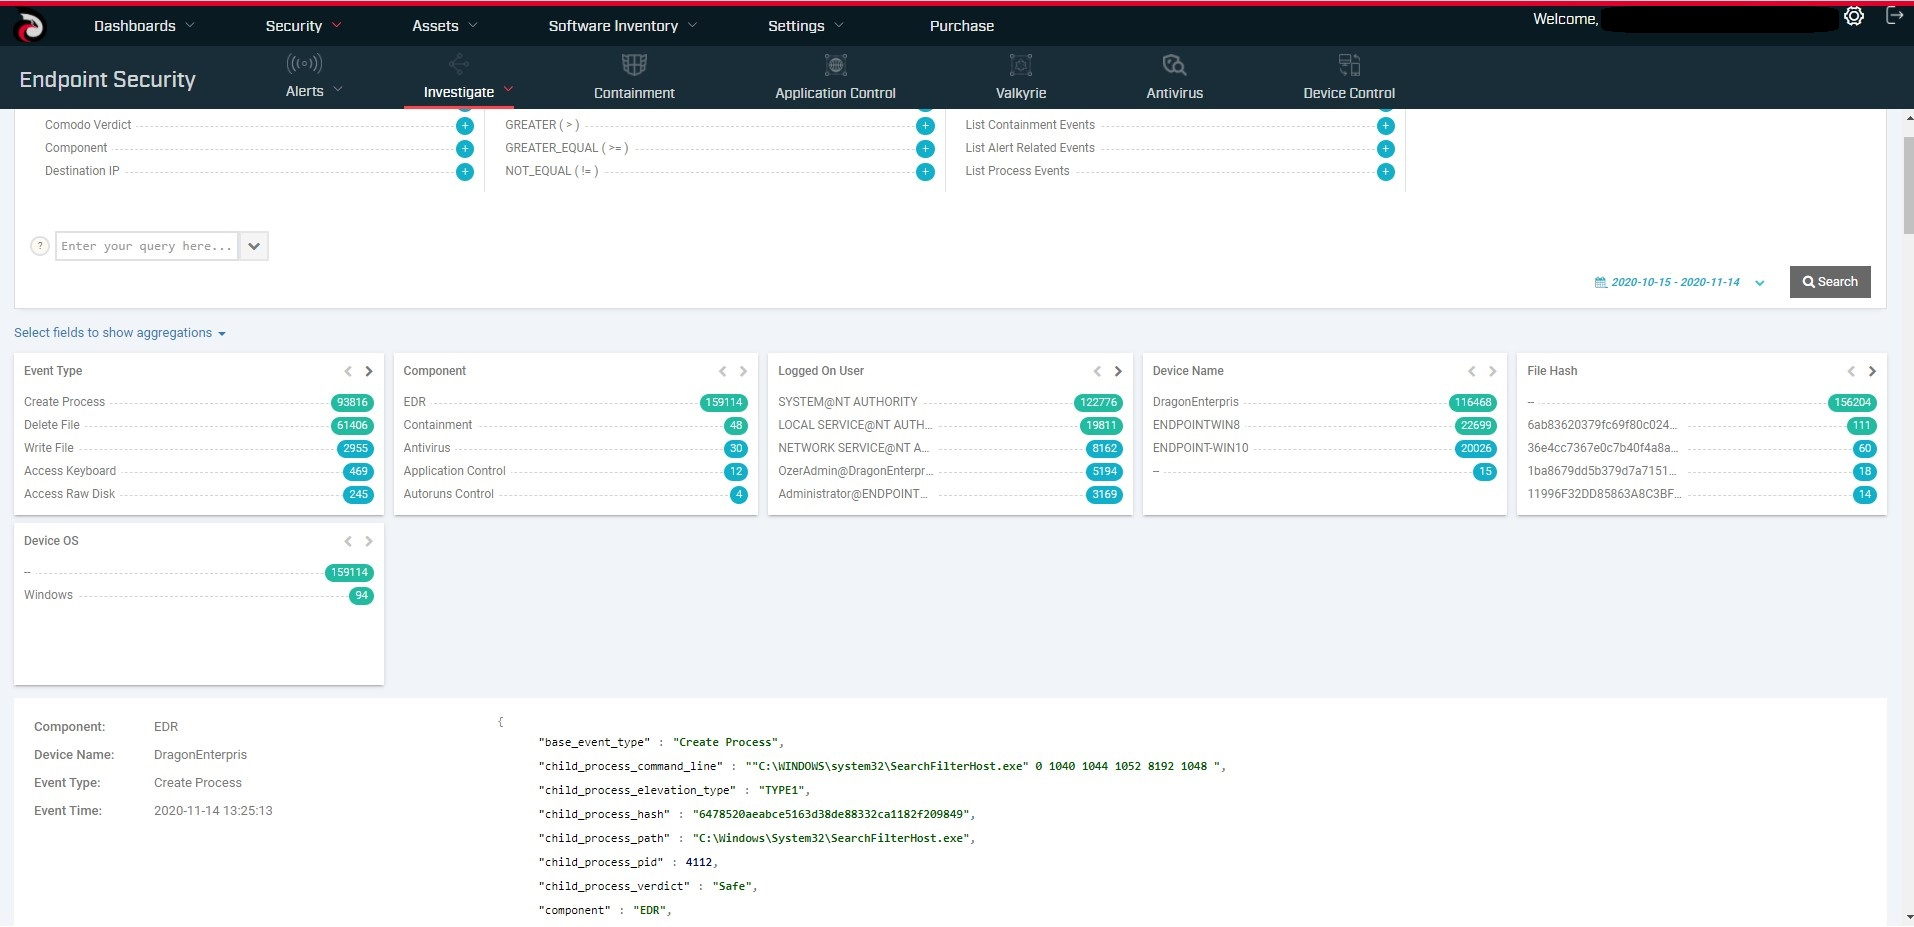
\includegraphics[width=1\textwidth]{Event-search.jpg}
    \caption{Event Search}
    \label{fig:event-search}
\end{figure}

\section{Benefits}
OpenEDR offers several benefits to organizations:
\begin{itemize}
    \item Enhanced security monitoring and incident response capabilities.
    \item Community-driven development for ongoing improvement.
    \item Detailed event analysis for accurate root cause identification.
    \item Simplified security architecture for multiple threat vectors.
    \item Real-time visibility and continuous analysis.
    \item Integration with the MITRE ATT\&CK framework for comprehensive security coverage.
\end{itemize}

\section{Conclusion}

Endpoint Detection and Response (EDR) solutions are vital components of modern cybersecurity strategies, offering a robust defense against a range of threats. In this report, we explored three key features of EDR that underscore its effectiveness in safeguarding organizations:

\begin{enumerate}
    \item Detection of Suspicious PowerShell Execution
    \item Detection of Clearing Security Log
    \item Detection of Writing a Fake System File
\end{enumerate}

These scenarios demonstrate the versatility and value of EDR in monitoring, detecting, and responding to security threats. EDR solutions play a pivotal role in identifying potential risks and enabling rapid response, enhancing an organization's overall security posture.

As the threat landscape continues to evolve, EDR remains a cornerstone of defense, offering continuous monitoring, real-time alerts, and actionable insights. Organizations are encouraged to harness the full capabilities of EDR to protect their digital assets and data.

In conclusion, EDR solutions are indispensable tools in the fight against cyber threats. By effectively deploying and leveraging the capabilities of EDR, organizations can bolster their defenses and mitigate the impact of security incidents. As cybersecurity challenges persist, EDR remains an essential ally in the quest for digital resilience and data protection.


\end{document}
